This chapter provides an overview of the \gls{acr:oqe}, 
its structure and the processes adopted for its development. 
A particular emphasis is placed on transparency, reproducibility,
community-based development and testing \parencite{pagani2014}, 
tenets endorsed since the early stages of development which make
the \gls{acr:oqe} indubitably characteristic. 
%
% ..............................................................................
\section{Overview of the OpenQuake-engine}
%
The \gls{acr:oqe} is an open-source hazard and risk calculation engine 
whose development is actively supported by the 
\href{http://globalquakemodel.org}{\gls{acr:gem}} initiative.
%
The \gls{acr:oqe} is part of a suite of open source software developed by 
\href{http://globalquakemodel.org}{\gls{acr:gem}} which comprises: the 
\gls{acr:oqe}, the OpenQuake-platform and a large set of tools of which 
the most interesting from a hazard perspective are the hazard modellers' 
toolkit (see \href{https://github.com/GEMScienceTools/hmtk}
{https://github.com/GEMScienceTools/hmtk}).

The development of the engine - started in 2010 and currently in 
progress - follows classical standards adopted for the development 
of open source software such as open access of the source code though an easily
accessible website and transparency of the development process\footnote{See for 
example the documentation available on the website 
of the \href{http://opensource.org/osr}{Open Source Initiative for a 
more comprehensive description of the development standards commonly 
adopted within the open source software community}}.
The engine was designed to operate on hardware with different properties
ranging from a simple laptop to a heterogeneous cluster of multi-core machines.
The operative system currently supported is Ubuntu Linux (additional
information on the supported version and on the installation procedure can 
be found on the GEM area on github, accessible at the following link:
\href{https://github.com/gem/oq-engine}{https://github.com/gem/oq-engine}). 
% . . . . . . . . . . . . . . . . . . . . . . . . . . . . . . . . . . . > Figure
\begin{figure}[!ht]
\centering
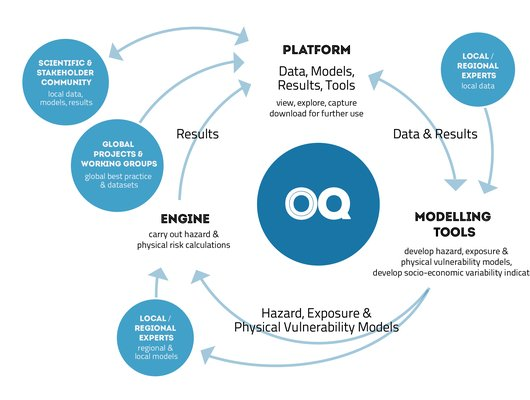
\includegraphics[width=14cm]{./Pictures/intro/OQ-workflows.jpg}
\caption{A schematic describing the OpenQuake suite.}
\label{fig:oq_platform}
\end{figure}
% . . . . . . . . . . . . . . . . . . . . . . . . . . . . . . . . . . . < Figure
%
% . . . . . . . . . . . . . . . . . . . . . . . . . . . . . . . . . . . . . . .
\subsection{Structure of the OpenQuake-engine}
The \gls{acr:oqe} is the combination of different and sometimes 
self-sufficient libraries. Below we provide a short description for each of
them.
\begin{description}
    \item [oq-hazardlib] Contains the software used to describe 
        seismic sources, create the \gls{acr:erf}, calculate hazard curves, 
        create stochastic event sets, compute ground motion fields and 
        calculate seismic hazard disaggregation.
    \item [oq-risklib] Comprises the used to describe exposures, vulnerability 
        and fragility curves and to compute losses.
    \item [oq-nrmllib] Includes the scheme which describes the structure of 
        the \gls{acr:oqe} input and output files. The majority of these files 
        is formatted according to a dialect of 
        \href{http://www.w3.org/XML/}{XML} called \gls{acr:nrml}. 
    \item [oq-commonlib] Includes common code for \gls{acr:oqe} applications,
        such as - for example - the code used to describe logic tree structures.
    \item [oq-engine] It incorporates the core of the \gls{acr:oqe}; the code in
        this library is the glue that sticks the different libraries together 
        and let the user easily perform calculations according to a established 
        set of calculation options.
\end{description}
%
% ..............................................................................
\section{Overview of the OpenQuake-engine development process}
%
The \gls{acr:oqe} is developed through a close and continuous collaboration 
between the GEM scientific and IT teams. The development process is completely
carried out in the open in order to favor and promote the
participation of experts working in organizations different from the GEM 
Foundation.
%
% . . . . . . . . . . . . . . . . . . . . . . . . . . . . . . . . . . . . . . .
\subsection{Development tools}
%
The \gls{acr:oqe} development process is completely open and transparent. Each
new feature, improvement or bug fix before being implemented is described 
in a bug tracking system (in our case, 
\href{https://launchpad.net/}{Launchpad}).  

The tools used to maintain and make publicly available the \gls{acr:oqe} 
master repository and to manage the almost ceaseless process improvement 
and expansion are \href{http://git-scm.com/}{git} and a git-based repository 
hosting service called \href{http://github.com/}{GitHub}.
%
\begin{table}[!t]
\centering
\begin{tabular}{p{4cm}p{9cm}}
\hline
\rowcolor{anti-flashwhite}
\bf{Service} & \bf{Link}  \\
\hline 
OQ-engine main website & 
    \href{http://www.globalquakemodel.org/openquake/start/engine/}
        {http://www.globalquakemodel.org/openquake/start/engine/} \\
OQ-engine bug tracking system & 
    \href{https://launchpad.net/openquake}{https://launchpad.net/openquake} \\
OQ-engine web repository & 
    \href{http://github.com/gem}{http://github.com/gem} \\
\hline
\end{tabular}
\caption{Main services and websites related to the \gls{acr:oqe}}
\end{table}
%
% . . . . . . . . . . . . . . . . . . . . . . . . . . . . . . . . . . . . . . .
\subsection{Programming language}
The core of the \gls{acr:oqe} is developed in 
\href{https://www.python.org/}{Python}. Python is a high level and open 
source programming language extensively used in the scientific community 
which can run on almost all the operative systems currently available.
%
% . . . . . . . . . . . . . . . . . . . . . . . . . . . . . . . . . . . . . . .
\subsubsection{Main libraries to which the \gls{acr:oqe} depends upon}
The development of the engine is using relying on a number of libraries such 
as:
\begin{description}
    \item [\href{http://redis.io/}{Redis}] A key-value store
    \item [\href{https://www.rabbitmq.com/}{RabbitMQ}] A messaging system
    \item [\href{http://www.celeryproject.org/}{Celery}] An asynchronous 
        task queue/job queue.
\end{description}
%
% ..............................................................................
\section{The basics of the OpenQuake-engine hazard component}
%
The hazard component of the \gls{acr:oqe} has been developed mostly following 
an object oriented programming paradigm taking in some cases as an example 
concepts introduced in the development of OpenSHA, a seismic hazard 
analysis library developed within a joint SCEC-USGS collaboration 
\parencite{field2003}. 

From a conceptual point of view, the main objects adopted in the development
of the oq-hazardlib follows quite closely the classical schematic proposed by
\textcite{reiter1991} i.e. a seismic source, a ground shaking intensity model 
and a calculator that using this information computes the hazard at the site.

The \gls{acr:oqe} builds on top of this library and expands this concept by
taking into account not just the essential objects needed to compute the hazard
at a site but also the associated epistemic uncertainties.
%
% . . . . . . . . . . . . . . . . . . . . . . . . . . . . . . . . . . . . . . .
\subsection{Calculation workflows}
The hazard component of the \gls{acr:oqe} provides four main calculation 
workflows:
\begin{itemize}
\item Classical \gls{acr:psha}. Calculates hazard curves, hazard maps, 
    and uniform hazard spectra by solving the PSHA integration procedure, 
    as proposed by \citetext{field2003}. 
    This is the usual approach adopted in regional/national-scale hazard 
    assessment, as well as in site-specific studies. Using the risk 
    component of the OQ-engine, the computed hazard curves can be 
    combined with a vulnerability and exposure model to derive 
    asset-specific loss exceedance curves and loss maps for various 
    return periods. Such analyses are useful for comparative risk 
    assessment between assets at different locations, or to understand
    the areas where mitigation actions should be concentrated. 
    Crowley and Bommer (2006) suggest this methodology tends to 
    overestimate losses at high return periods for portfolios of 
    structures and recommend the use of methods capable to account 
    for the spatial correlation of ground motion residuals.
\item Event-based \gls{acr:psha}. Computes stochastic event sets (i.e., 
    synthetic catalogs of earthquake ruptures) and ground-motion fields 
    for each rupture, possibly taking into account the spatial 
    correlation of within-event residuals. This is essentially a 
    Monte Carlo–based PSHA calculator \parencite{musson2000}. The computed 
    synthetic catalogs can be used for comparisons against a real 
    catalog, whereas hazard curves and hazard maps can be derived from 
    post- processing the ground-motion fields \parencite{ebel1999}. 
    Ground-motion fields are essential input for loss estimations, 
    whereby loss exceedance curves and loss maps are calculated for 
    a collection of assets by combining a vulnerability and exposure
    model with these sets of ground- motion fields. Because the spatial
    correlation of the ground-motion residuals can be taken into account
    in this calculator, the losses to each asset can be summed per 
    ground-motion field, and a total loss exceedance curve representative 
    of the whole collection of assets can be derived. These results are 
    important for deriving reliable estimates of the variance of the
    total losses.
\item Scenario-based \gls{acr:sha}. Given an earthquake rupture and a 
    ground-shaking model, a set of ground-motion fields can be computed. 
    This is a typical use case for urban-scale loss analysis. This set of
    ground-motion fields can be em- ployed with a fragility/vulnerability 
    model to calculate distribution of damage/losses for a collection of
    assets. Such results are of importance for emergency management planning
    and for raising societal awareness of risk.
\item Disaggregation. Given a PSHA model, it computes the earthquake
    scenarios contributing the most to a given hazard level at a specific
    site \parencite{bazzurro1999}. Currently this is done following 
    the classical PSHA methodology; this functionality will be added to 
    the event-based calculator in subsequent development phases.
\end{itemize}
%
% . . . . . . . . . . . . . . . . . . . . . . . . . . . . . . . . . . . . . . .
\subsection{Testing and Quality Assurance}
%
\gls{acr:qa} is an aspect carefully considered in the development 
of the \gls{acr:oqe} based on several important motivations.
%
The first and most practical one is dictated by the development process which 
involves experts from different disciplines (e.g. seismic hazard and 
information technology). 
%
In this context the use of a common and strong testing process is a way 
trough which developers confirm the compliance of the tools developed 
against the requirements defined by the scientific team and it is also 
a process through which it can be demonstrated that the entire code fulfills 
minimum quality criteria (e.g. the code comply with the
\href{http://legacy.python.org/dev/peps/pep-0008/}{PEP 8 standard}, the code
before getting into the master repository is revised by at least one one 
separate developer and is clearly documented).
% 
The second motivation relates to the specific goal of building a dynamical 
tool (i.e. providing a very large flexibility) while constantly proving the 
stability and reliability of the supported calculation workflows.

The implementation of tests is usually done in parallel with code 
development, but tests are also added every time there's a bug fix 
in order to improve the overall robustness and reliability of the code.
%
Four are the approaches used to test the \gls{acr:oqe} behavior 
and therefore provide high quality assurance standards. 
%
\begin{description}
    \item [Unit-testing] A testing methodology which checks discrete 
        units of code against associated control data, expected behaviors 
        and operating procedures. A special set of unit-tests are the ones
        systematically created for every \gls{acr:gsim} implemented 
        (additional information about this specific topic is available within 
        Chapter \ref{chap:gmpes})
    \item [Testing against benchmark results] The results provided by the 
        \gls{acr:oqe} are compared benchmark results. Several of the 
        tests defined by \textcite{thomas2010} are used to check the 
        reliability and correctness of the results provided. 
    \item [Tests against provided by other PSHA codes: simple cases]
    \item [Tests against provided by other PSHA codes: national or regional 
        PSHA input models]
\end{description}
%
% ..............................................................................
\section{Input and output description}
The \gls{acr:oqe} reads and writes for the majority XML formatted files
according to a

%
% ..............................................................................
\section{Description of book structure}
This book is organised into five additonal chapters. Chapter 2 contains a 
short introduction to seismic hazard analysis with a focus on probabilistic 
methodologies and on their implementation into the OQ-engine.
